\documentclass[a4paper,11pt]{book}

\usepackage[utf8]{inputenc}

\usepackage[spanish]{babel}\decimalpoint

\usepackage{graphicx}
    \graphicspath{{resources/}}
\usepackage{pdflscape}

\usepackage{amsmath}

\usepackage{listings}
\usepackage{dcolumn}
    \newcolumntype{.}{D{.}{\esperiod}{-1}}
    \makeatletter
    \addto\shorthandsspanish{\let\esperiod\es@period@code}
    \makeatother
    \RequirePackage{verbatim}
\usepackage{fancyhdr}
    \pagestyle{fancy}
    \fancyhf{}
    \fancyhead[LO]{\leftmark}
    \fancyhead[RE]{\rightmark}
    \fancyhead[RO,LE]{\textbf{\thepage}}
\usepackage{afterpage}
\usepackage{longtable}
    \usepackage{array}
\usepackage{hyperref}
    \hypersetup{
        pdfauthor = {Jose Manuel García Cazorla (jmgarcaz@correo.ugr.es)},
        pdftitle = {Aplicación de control para testeador de faros de vehículos},
        pdfkeywords = {firmware, microcontrolador, Arduino, PWM, aplicación, frontend, C, Python, QT},
        pdfproducer = {pdflatex}
    }
\usepackage{url}
\usepackage{colortbl}
\usepackage[stable]{footmisc}
\usepackage{pdfpages}
\usepackage[fixlanguage]{babelbib}

\renewcommand{\chaptermark}[1]{\markboth{\textbf{#1}}{}}
\renewcommand{\sectionmark}[1]{\markright{\textbf{\thesection. #1}}}

\setlength{\headheight}{1.5\headheight}

\newcommand{\HRule}{\rule{\linewidth}{0.5mm}}

\newtheorem{teorema}{Teorema}[chapter]
\newtheorem{ejemplo}{Ejemplo}[chapter]
\newtheorem{definicion}{Definición}[chapter]

\definecolor{gray97}{gray}{.97}
\definecolor{gray75}{gray}{.75}
\definecolor{gray45}{gray}{.45}
\definecolor{gray30}{gray}{.94}

\lstset{
    frame=Ltb,
    framerule=0.5pt,
    aboveskip=0.5cm,
    framextopmargin=3pt,
    framexbottommargin=3pt,
    framexleftmargin=0.1cm,
    framesep=0pt,
    rulesep=.4pt,
    backgroundcolor=\color{gray97},
    rulesepcolor=\color{black},
    %
    stringstyle=\ttfamily,
    showstringspaces = false,
    basicstyle=\scriptsize\ttfamily,
    commentstyle=\color{gray45},
    keywordstyle=\bfseries,
    %
    numbers=left,
    numbersep=6pt,
    numberstyle=\tiny,
    numberfirstline = false,
    breaklines=true
}

\lstnewenvironment{listing}[1][]
    {\lstset{#1}\pagebreak[0]}{\pagebreak[0]}

    \lstdefinestyle{CodigoC}{
        basicstyle=\scriptsize,
        frame=single,
        language=C,
        numbers=left
    }
    \lstdefinestyle{CodigoC++}{
        basicstyle=\small,
        frame=single,
        backgroundcolor=\color{gray30},
        language=C++,
        numbers=left
    }
    \lstdefinestyle{Consola}{
        basicstyle=\scriptsize\bf\ttfamily,
        backgroundcolor=\color{gray30},
        frame=single,
        numbers=none
    }
\newcommand{\bigrule}{\titlerule[0.5mm]}

\makeatletter
\def\clearpage{
    \ifvmode
        \ifnum \@dbltopnum =\m@ne
            \ifdim \pagetotal <\topskip
                \hbox{}
            \fi
        \fi
    \fi
    \newpage
    \thispagestyle{empty}
    \write\m@ne{}
    \vbox{}
    \penalty -\@Mi
}
\makeatother


\begin{document}

    \begin{titlepage}
    \newlength{\centeroffset}
    \setlength{\centeroffset}{-0.5\oddsidemargin}
    \addtolength{\centeroffset}{0.5\evensidemargin}
    \thispagestyle{empty}

    \noindent\hspace*{\centeroffset}

    \begin{minipage}{\textwidth}
        \centering

        
\includegraphics[width=0.9\textwidth]{logo_ugr.jpg}\\[1.4cm]

        \textsc{\Large TRABAJO FIN DE GRADO\\[0.2cm]}
        \textsc{INGENIERÍA INFORMÁTICA}\\[1cm]

        \Huge\bfseries Aplicación de control para testeador de faros de vehículos
    \end{minipage}

    \vspace{2.5cm}
    \noindent\hspace*{\centeroffset}

    \begin{minipage}{\textwidth}
        \centering

        \textbf{Autor}\\{Jose Manuel García Cazorla}\\[2.5ex]
        \textbf{Directores}\\{Andrés María Roldán Aranda}\\[2.5ex]

        
\includegraphics[width=0.3\textwidth]{etsiit_logo.png}\\[0.1cm]

        \textsc{Escuela Técnica Superior de Ingernierías Informática y de Telecomunicación}\\
        \textsc{---}\\
        Granada, Septiembre de 2025
    \end{minipage}
\end{titlepage}


    \begin{titlepage}
    \setlength{\centeroffset}{-0.5\oddsidemargin}
    \addtolength{\centeroffset}{0.5\evensidemargin}
    \thispagestyle{empty}

    \noindent\hspace*{\centeroffset}

    \begin{minipage}{\textwidth}
        \centering
        \vspace{3.3cm}

        
\includegraphics{granasat_logo.png}
        \vspace{0.5cm}

        \Huge\bfseries Aplicación de control para testeador de faros de vehículos
    \end{minipage}

    \vspace{2.5cm}
    \noindent\hspace*{\centeroffset}

    \begin{minipage}{\textwidth}
        \centering

        \textbf{Autor}\\{Jose Manuel García Cazorla}\\[2.5ex]
        \textbf{Directores}\\{Andrés María Roldán Aranda}\\[2cm]
    \end{minipage}

    \vspace{\stretch{2}}
\end{titlepage}


    \cleardoublepage
    \thispagestyle{empty}

    \begin{center}
    \large\bfseries Aplicación de control para testeador de faros de vehículos
\end{center}

\begin{center}
    Jose Manuel García Cazorla\\
\end{center}

\noindent{\textbf{Palabras clave}: firmware, microcontrolador, Arduino, PWM, aplicación, frontend, C, Python, QT}\\

\vspace{0.7cm}
\noindent{\textbf{Resumen}}\\

La industria del automóvil es un sector en constante desarrollo, siempre a la vanguardia de los avances tecnológicos para producir vehículos cada vez más sofisticados. Tratándose del medio de transporte más usado en la actualidad, cada pieza es sumamente importante: por muy prescindible que parezca, puede llegar a salvar vidas.

Uno de los componentes que más se pueden dan por sentado son los faros. Aunque se usen solo una fracción del tiempo total que pasamos al volante, sin ellos no podríamos conducir de noche, o en situaciones en las que la visibilidad no sea óptima.

En este trabajo se presenta el análisis, diseño y desarrollo del firmware de PWM Box, un dispositivo que genera señales PWM configurables por el usuario con el objetivo de probar faros de vehículos. Asimismo, se implementa una interfaz gráfica que permite gestionar distintos perfiles y parámetros de configuración del dispositivo desde un ordenador.

\cleardoublepage

\thispagestyle{empty}

\begin{center}
    Control app for a vehicle headlight tester
\end{center}

\begin{center}
    Jose Manuel García Cazorla\\
\end{center}

\noindent{\textbf{Keywords}: firmware, microcontroller, Arduino, PWM, app, frontend, C, Python, QT}\\

\vspace{0.7cm}
\noindent{\textbf{Abstract}}\\

The car industry is an ever-developing sector, always on the cutting edge of technological advances to produce increasingly sophisticated vehicles. Currently being the most used means of transportation, each of its components is extremely important: no matter how expendable it seems, it may even help to save lives.

One of the most easily overlooked components are headlights. Even though we only use them for a fraction of the time we spend on our cars, we wouldn't be able to drive at night or in low-visibility situations without them.

This project showcases the analysis, design and development of the firmware for the PWM Box, a device that generates user-configurable PWM signals intended for testing vehicle headlights. Additionally, a graphic interface is implemented, which allows to manage the device's profiles and other configuration parameters from a computer.

\chapter*{}
\thispagestyle{empty}

\noindent\rule[-1ex]{\textwidth}{2px}\\[4.5ex]

Yo, \textbf{Jose Manuel García Cazorla}, alumno del Grado en Ingeniería Informática de la \textbf{Escuela Técnica Superior de Ingernierías Informática y de Telecomunicación de la Universidad de Granada}, con DNI 15434710P, autorizo la ubicación de la siguiente copia de mi Trabajo de Fin de Grado en la biblioteca del centro para que pueda ser consultada por las personas que lo deseen.

\vspace{6cm}

\noindent Fdo.: Jose Manuel García Cazorla

\vspace{2cm}

\begin{flushright}
    Granada, a 1 de Septiembre de 2025.
\end{flushright}

\chapter*{}
\thispagestyle{empty}

\noindent\rule[-1ex]{\textwidth}{2px}\\[4.5ex]

D. \textbf{Andrés María Roldán Aranda}, Profesor del área de TODO del Departamento de Electrónica y Tecnología de Computadores de la Universidad de Granada.

\vspace{0.5cm}

\textbf{Informan:}
Que el presente trabajo, titulado \textit{\textbf{Aplicación de control para testeador de faros de vehículos}}, ha sido realizado bajo su supervisión por \textbf{Jose Manuel García Cazorla}, y autorizamos la defensa de dicho trabajo ante el tribunal que corresponda.

\vspace{0.5cm}

Y para que conste, expiden y firman el presente informe en Granada a 1 de Septiembre de 2025.

\vspace{1cm}

\textbf{El director:}

\vspace{5cm}

\noindent\textbf{Andés María Roldán Aranda}

\chapter*{Agradecimientos}
\thispagestyle{empty}

\vspace{1cm}

% Doy las gracias a Andrés, mi tutor de este Trabajo de Fin de Grado, por guiarme en esta dura etapa.

% Agradecer también a mi familia y a mi pareja por su incondicional apoyo y ánimos a lo largo de este proceso. Sin ellos, me habría sido imposible alcanzar este logro.


    \frontmatter
    \tableofcontents
    \listoffigures
    \listoftables

    \mainmatter
    \setlength{\parskip}{5pt}

    % \chapter
    % \section
    % \subsection
    % \subsubsection
    % \paragraph
    % \subparagraph

    \chapter{Introducción}
\label{ch:introduccion}

Como es costumbre, esta memoria merece ser empezada por el principio: el ``qué'' y el ``por qué'' de este proyecto. Esa es la función que cumplirá esta introducción, en la que se contextualizarán los aspectos fundamentales del trabajo, así como la motivación detrás de su realización. A partir de ellos, se definirán los objetivos específicos que se tratarán de cumplir, y por último se describirá brevemente la estructura de este documento.

\section{Contexto}

Un microcontrolador es un circuito integrado programable que está compuesto de distintos bloques funcionales que cumplen tareas específicas. Este incluye en su interior los tres componentes esenciales de un ordenador (una CPU, memoria y mecanismos de entrada y salida), conviertiéndolo funcionalmente en un ordenador a pequeña escala.

A pesar de su tamaño, son muy potentes, consumiendo menos energía que un ordenador convencional y a un precio mucho más bajo. Esto permite integrarlos en todo tipo de dispositivos, desde electrodomésticos o teléfonos móviles hasta aquellos usados en la automatización industrial y en la industria aeroespacial. Hoy en día son esenciales para muchas de las tareas que realizamos de manera cotidiana.

Sin embargo, a pesar de sus numerosos beneficios, sus recursos son limitados, lo cual los hace menos apropiados para aplicaciones que necesiten una mayor cantidad de memoria o de procesamiento. Es por ello que usarlos de forma conjunta con un ordenador tradicional puede ser un factor clave en algunos casos.

\section{Motivación}
\label{sec:motivacion}

Este proyecto se realiza a partir de la necesidad de Valeo, una empresa distribuidora en el ámbito automobilístico, de proporcionar a sus fabricantes una forma de probar el funcionamiento de los faros de distintos vehículos.

El laboratorio de GranaSAT, del que el tutor de este trabajo forma parte, fue el encargado de proporcionar una solución a dicha urgencia: usar un dispositivo basado en un microcontrolador para producir las señales PWM que alimentan dichos faros.

Esta ha sido presentada como Trabajo de Fin de Grado en años anteriores. Primero por Luis Sánchez, autor de la PCB y de todo el apartado electrónico, y luego por Rubén Sánchez, que se encargó de desarrollar el firmware del dispositivo.

Este dispositivo, al que llamamos PWM Box, ha sido usado por Valeo de forma satisfactoria. Sin embargo, se han vuelto a poner en contacto con GranaSAT para expresar una nueva necesidad: la capacidad de almacenar distintos perfiles de configuración para el dispositivo.

Para ello, se plantea en este trabajo la implementación de nuevas funcionalidades en el dispositivo que permitan resolver esta cuestión. Asimismo, se pretende proporcionar a la empresa una interfaz gráfica que les permita gestionar estas configuraciones sin tener que depender exclusivamente de la limitada memoria del microcontrolador.

A su vez, esta tarea es idónea para complementar las competencias que he adquirido a lo largo de la mención de Ingeniería de Computadores del Grado. Por un lado, me permite poner en práctica lo aprendido en un proyecto real, mientras que por otro, constituye una forma de acercarme a un desarrollo algo más a alto nivel.

% \section{Conocimientos previos}
% \label{sec:conocimientos}
%
% En la realización de este trabajo se han puesto en práctica competencias adquiridas en distintas asigntauras de la titulación, y más concretamente de la rama que he cursado, \emph{Ingeniería de Computadores}. Por nombrar algunas:
%
% \begin{itemize}
%     \item\textbf{Fundamentos y Metodología de la Programación:} Tratándose de un trabajo de desarrollo, se deben mencionar las asignaturas del Grado en las que se establecen los pilares del conocimiento en programación de muchos estudiantes. Desde lo más básico hasta conceptos más complejos, una gran parte de su contenido se ha aplicado en el desarrollo de este TFG.
%     \item\textbf{Estructuras de Datos:} Como su nombre indica, se centra en los distintos contenedores de datos (vectores, colas, pilas, etc), sus particularidades, y cómo trabajar con ellos, conocimientos que han sido de gran utilidad a lo largo de este proyecto.
%     \item\textbf{Sistemas con Microprocesadores:} Esta asignatura sirve de introducción a numerosos aspectos de la programación de microcontroladores, culminando en la construcción de un robot de lucha usando un Arduino. Todo ello ha sido puesto en práctica para desarrollar el firmware expuesto.
%     \item\textbf{Sistemas Empotrados:} Complementa a la anterior, entrando más en detalle en la arquitectura de los microcontroladores, y aún a más bajo nivel. Aporta conocimientos que han sido de gran valor a lo largo de este proyecto.
% \end{itemize}

\section{Objetivos}
\label{sec:objetivos}

A continuación se definen los requisitos generales y específicos de este TFG, obtenidos a partir del contexto proporcionado en esta introducción.

\begin{itemize}
    \item\textbf{OG-1.} Mejorar el actual firmware del PWM Box.
    \begin{itemize}
        \item\textbf{OE-1.1.} Realización de una ingeniería inversa de la versión actual del firmware, con el objetivo de localizar y corregir posibles errores existentes.
        \item\textbf{OE-1.2.} Desarrollar una funcionalidad que permita la utilización de la memoria EEPROM del microcontrolador para almacenar perfiles de configuración.
        \item\textbf{OE-1.3.} Incluir un nuevo modo de funcionamiento que permita probar faros que requieran señales de una frecuencia inferior a la que el dispositivo es capaz de generar.
    \end{itemize}
    \item\textbf{OG-2.} Implementación de una interfaz gráfica complementaria.
    \begin{itemize}
        \item\textbf{OE-2.1.} Integrar la aplicación con el dispositivo, permitiendo el intercambio de información entre ambos.
        \item\textbf{OE-2.2.} Implementar los mecanismos necesarios para permitir el envío de perfiles de configuración desde la interfaz al PWM Box.
        \item\textbf{OE-2.3.} Incluir en la interfaz elementos que permitan visualizar y modificar las distintas configuraciones que esta almacene.
        \item\textbf{OE-2.4.} Permitir la exportación e importación de perfiles de la interfaz al disco del ordenador.
    \end{itemize}
\end{itemize}

Se determinan, adicionalmente, los siguientes objetivos de aprendizaje:

\begin{itemize}
    \item\textbf{OA-1.} Poner en práctica en un proyecto real los conociemientos adquiridos durante el Grado acerca de la programación a bajo nivel.
    \item\textbf{OA-2.} Aprender sobre el diseño y desarrollo de una aplicación de escritorio.
    \item\textbf{OA-3.} Adquirir destreza en algún lenguaje de programación que no haya usado durante la carrera.
    \item\textbf{OA-4.} Llevar a cabo la integración de distintos sistemas independientes en un mismo producto final.
\end{itemize}

% El objetivo general de este TFG es mejorar el firmware de la versión existente del dispositivo, al que llamaremos \emph{PWM Box}, corrigiendo algunos errores presentes en ella y añadiendo nuevas funcionalidades. Además, se plantea la implementación de una interfaz gráfica compatible con Windows y Linux, que permita el almacenamiento y gestión de distintos perfiles de configuración para el dispositivo.
%
% A raíz de este, se han concretado otros objetivos más definidos:
%
% \begin{itemize}
%     \item\textbf{Ingeniería inversa de la versión actual:} Análisis en profundidad el estado actual del dispositivo, entendiendo su funcionamiento e identificando posibles mejoras a implementar.
%     \item\textbf{Almacenamiento de perfiles en el microcontrolador:} Utilización de la memoria EEPROM del microcontrolador para almecenar datos que convenga mantener de forma no volátil.
%     \item\textbf{Funcionalidad compatible con faros de baja velocidad:} Implementación de un nuevo modo de funcionamiento que permita también probar faros de baja velocidad, es decir, que requieran señales de una frecuencia inferior a las que el dispositivo está programado para producir.
%     \item\textbf{Interfaz gráfica:} Diseño de una aplicación para ordenador que permita gestionar la configuración del dispositivo tanto desde Windows como desde Linux. Esta ha de ser capaz de obtener las configuraciones almacenadas en el PWM Box, guardarlas de forma permanente en el disco, y posteriormente volver a cargarlas en el dispositivo.
% \end{itemize}

\section{Estructura del documento}

Este documento se divide en distintos apartados, centrándose cada uno en un aspecto distinto del tema que trata:

\begin{itemize}
    \item\textbf{Introdución:} El primer apartado, en el cual nos encontramos, sirve de introducción al proyecto. Proporciona información general del desarrollo que se va a abordar, proporcionando contexto y definiendo a grandes rasgos las tareas que se esperan cumplir.
    \item\textbf{Estado del arte:} En segundo lugar, se realizará un análisis del estado del proyecto antes de empezar a trabajar en él. Se tratará de describir de forma detallada las características de las versiones anteriores del firmware, identificando áreas en las que mejorar y comenzando a tomar algunas decisiones de cara a la propuesta.
    \item\textbf{Planificación temporal:} En este apartado se describirá la metodología seguida para llevar a cabo el trabajo, planificando de antemano cuánto tiempo invertir en cada una de sus partes.
    \item\textbf{Firmware:} Constituye el principio de la propuesta. En él se desarrollan las distintas fases en las que se ha decidido enfrentar esta parte del proyecto.
    \item\textbf{Interfaz:} Segunda parte de la propuesta, en la que se abordan los distintos aspectos definidos para la implementación de la interfaz gráfica.
    \item\textbf{Presupuesto:} En este apartado se realiza una breve estimación del coste total del desarrollo del proyecto, desglosado según su procedencia.
    \item\textbf{Conclusiones y trabajo futuro:} Finalmente, se concluirá la memoria reflexionando sobre el cumplimiento de los objetivos fijados. También se mencionarán algunos aspectos en los que se considera que hay cabida para mejoras, en caso de que continúe trabajando en el proyecto.
\end{itemize}



    \chapter{Estado del arte}
\label{ch:estado_del_arte}

Como se ha comentado en la \autoref{sec:motivacion}, este trabajo continúa el comenzado por el alumno Rubén Sanchez en cursos anteriores. Por ello, el primer paso a realizar al revisar el estado del arte es una ingeniería inversa de su desarrollo, con el fin de identificar tanto sus fortalezas como sus puntos débiles.
\section{Ingeniería inversa}
\label{sec:inginv}

Para este proceso, se recibe por parte del tutor un archivo comprimido con el código existente del proyecto, así como el prototipo actual del dispositivo, mostrado anteriormente en la \autoref{sec:motivacion}.

\begin{figure}[ht]
    \centering
    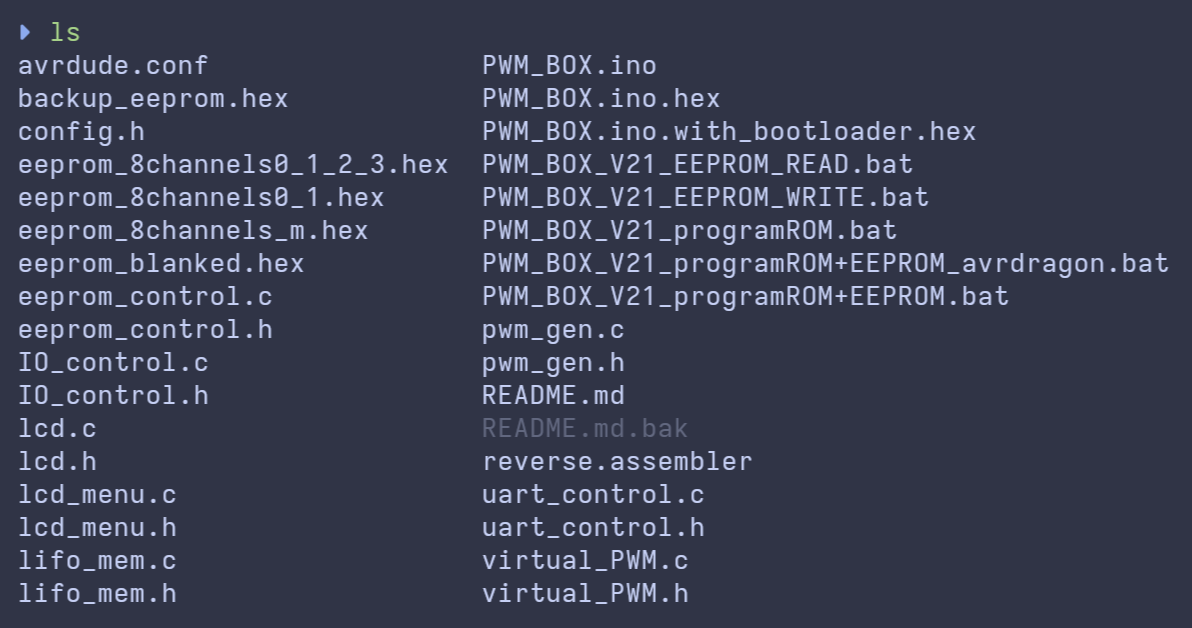
\includegraphics[width=0.8\textwidth]{fw_files_v0.png}
    \caption{Contenido de \textit{PWM\_BOX.RAR}.}
    \label{fig:fw_v0}
\end{figure}

Con estos últimos, se procede a realizar una primera clasificación básica para facilitar su manejo. Según su contenido y utilidad, se pueden distinguir los distintos tipos de archivos:

\begin{itemize}
    \item{\textbf{Archivos HEX:}} Estos contienen datos en formato hexadecimal. Por el nombre, se pueden distinguir entre los que contienen datos para la memoria no volátil del microcontrolador (EEPROM), y los que contienen el programa en sí.
    \item{\textbf{Archivos BAT:}} Se tratan de archivos de comandos para Windows. Examinando su contenido, se puede ver que todos ellos ejecutan comandos de un programa llamado AVRDUDE\footnote{\url{https://github.com/avrdudes/avrdude}}.\\
    AVRDUDE es una utilidad multiplataforma para la programación de microcontroladores AVR, entre los que se encuentran los usados por Arduino. Permite todo tipo de operaciones de carga y descarga de datos de las distintas memorias del microcontrolador. Es una herramienta usada muy comúnmente, funcionando incluso de \textit{back-end} en otros entornos de desarrollo.
    \item{\textbf{Archivos de código:}} Por un lado tendríamos las cabeceras y su implementación, en los usuales archivos H y C. Por otro lado, encontramos un archivo INO, que es el tipo usado por Arduino IDE para distinguir que se trata del archivo principal del proyecto. Este contiene las funciones \verb|setup()| y \verb|loop()|, que definen el flujo básico del programa: la primera se ejecuta una vez al inicio, y la segunda conforma el bucle principal de ejecución.
\end{itemize}

Con los archivos algo más organizados tras esta primera distinción, se pasa a hacer un análisis del código y de su funcionamiento, usando como apoyo la documentación de Rubén. Según la misma, se puede dividir el programa en distintos grupos:

\subsection{Archivo principal}

Consiste en el archivo principal INO que se mencionó anteriormente. En él, encontramos algunos elementos usados para determinar el flujo de ejecución del programa:

\begin{itemize}
    \item En primer lugar tenemos una cola de eventos, que recoje las acciones del usuario y permite al programa procesarlas en orden. Se desarrollará en una sección posterior.
    \item Un contador de tiempo, que mide cuánto lleva el usuario sin interactuar con el dispositivo para mostrar u ocultar un salvapantallas.
    \item El uso de distintas interrupciones para el manejo de la entrada del usuario, la generación de la señal PWM de salida y la comunicación por UART. % Esto último parece no estar implementado, puesto una gran parte del código se encuentra comentada, sin hacer referencia a ninguna función que lo maneje en su lugar.
\end{itemize}

Una cosa a comentar sobre el actual flujo del programa es el uso de interrupciones. Su uso es muy necesario para la generación de las señales PWM. Una interrupción se genera a una cierta frecuencia, y, dependiendo de los parámetros que introduzca el usuario, las señales cambian de estado cuando les corresponda. Esto asegura que los cambios se realizan en el momento preciso, mientras que si se gestionaran en el bucle principal, el momento exacto de las actualizaciones sería más incierto.

Sin embargo, la alta frecuencia de las interrupciones podría provocar una "sobrecarga" (\textit{interrupt overload}). Esta provocaría que otras tareas en ejecución, en este caso el bucle principal, no recibiera el suficiente tiempo de CPU, afectando al rendimiento. Esta condición puede también darse si, aun manteniendo un bajo número de interrupciones, las rutinas que estas ejecutan son demasiado largas.

Por todo ello, el uso de interrupciones para manejar la entrada de usuario a través del codificador rotatorio parece, tras un primer análisis, acertado. Su frecuencia será varias magnitudes menor que las destinadas a atender las señales de salida, de forma que no aportarán al problema anteriormente mencionado. Al mismo tiempo, se asegurarán de que ningún \textit{input} del usuario se pierde debido a que la CPU se encuentre ocupada. \cite{chapman}

\subsubsection{Buffer de eventos} Se trata de una cola circular estándar, en la que se van incluyendo datos de tipo evento. Estos consisten de un entero que determina el tipo de evento, junto a dos parámetros opcionales. Estos últimos parecen no ser utilizados en el resto del programa. Se distinguen eventos para giros del \textit{rotary encoder}, para su pulsación y para la llegada de datos a la UART.

El uso de un buffer de eventos aporta un mecanismo más para evitar la comentada sobrecarga por interrupciones. Con él, las funciones que las procesan pueden dedicarse únicamente a añadir el evento que corresponda a la cola, evitando rutinas demasiado largas. Será luego el bucle principal el que se encargue de ejecutar la acción vinculada al evento concreto, cuando la CPU pueda dedicarle tiempo.

% Las interrupciones también tienen sus ventajas para la comunicación por el puerto serie. No se sabe en qué punto llegará un mensaje al que atender, y realizar la comprobación en el bucle principal puede ralentizar otras partes del programa si el volumen de datos recibidos es muy alto. Generar una interrupción para atender a la UART sólo cuando ocurra la comunicación lo evita, y ayuda a prevenir errores en la recepción.

% Sin embargo, a la hora de gestionar la entrada del usuario a través del codificador rotatorio, su uso no parece tan necesario. Teniendo en cuenta el objetivo del dispositivo, lo esencial es asegurar que la señal PWM se genera con la configuración correcta. Las interrupciones continuas generadas por cada movimiento del \textit{rotary encoder} podrían generar un exceso de cambios de contexto que afecten al rendimiento general del programa.

% \subsection{Buffer circular}

% Aparece documentado con el nombre de \textit{memoria LIFO}. Se entiende que es una errata, puesto que al revisar el código se puede comprbar que se trata de un buffer circular, que funciona como una cola FIFO.

% Implementa las funciones estándar de una cola circular, que se usada en el programa, como se ha mencionado en la sección anterior, como buffer de eventos. Destaca también la definición de un dato de tipo evento, que permite distinguir entre movimiento hacia arriba, movimiento hacia abajo y pulsación del codificador rotatorio, además de entrada de mensaje en la UART.

% El uso de un buffer de eventos aporta un mecanismo más para evitar la sobrecarga de interrupciones comentada en la sección anterior. Con él, las rutinas para manejar las interrupciones pueden dedicarse únicamente a añadir el evento que corresponda a la cola. Será luego el bucle principal el que se encargue de ejecutar la acción vinculada al evento concreto, cuando la CPU pueda dedicarle tiempo.

% De este tipo evento cabe mencionar que parece estar inacabado, puesto que se define como una estructura en la que se puede opcionalmente incluir un argumento para algunos tipos de eventos, que sin embargo luego no se usa en el resto del programa.

\subsection{EEPROM}

Se trata de un archivo que sienta las bases para el guardado de datos en la memoria no volátil del microcontrolador. Este punto se distingue como uno de los que quedó fuera del desarrollo anterior, ya que únicamente aparecen implementadas algunas funciones básicas para leer posiciones determinadas de la memoria, que llaman directamente a otras de la librería de AVR.

De la breve implementación presente en este punto se puede comentar una cosa, y es que las lecturas y escrituras se están realizando proporcionando directamente la posición de memoria. Esto es un claro punto a mejorar, puesto que mantener estas posiciones guardadas puede ser tedioso, y disminuir la legibilidad del código. Una forma más apropiada de tratarlo sería definir la estructura de la memoria, de forma que los accesos a la misma puedan realizarse usando variables.

% Se define también un tipo de dato que, según la documentación, tiene la función de facilitar el traspaso de información a la memoria. % Sin embargo, no termino de entender su funcionamiento, puesto que se trata de una \verb|union| que agrupa distintas variables sin relación.

\subsection{Entrada/Salida}

% TODO: Mencionar que el rotary iba regular

En él se definen distintas funciones relacionadas con el codificador rotatorio y el manejo de eventos. También se distingue el prototipo de una función que serviría para decodificar un mensaje recibido por el puerto serie. Sin embargo, la lógica a bajo nivel del mismo no está implementada, por lo que actualmente no se le está dando uso.

De este módulo cabe destacar que el funcionamiento del \textit{rotary encoder} no es del todo correcto, generando en ocasiones dobles pulsaciones y no detectando algunos de los giros.

\subsection{LCD}

Se trata, con diferencia, del módulo más extenso de todo el programa. En él aparecen definidas distintas funciones que determinan el contenido de la pantalla según las acciones que vaya realizando el usuario. Podemos distinguir los siguientes menús:

\begin{itemize}
    \item\textbf{Lista:} Es el menú principal del sistema. En él se muestran las diferentes señales a configurar, así como las opciones de guardar y cargar configuraciones en la EEPROM (no operativas aún).
    \item\textbf{PWM:} Permite la configuración de los 4 parámetros principales del PWM que se seleccione en la pantalla anterior.
    \item\textbf{Contraseña:} Permite bloquear algunas características del dispositivo, como las que alteran el estado de la memoria EEPROM, tras una contraseña, evitando el acceso de usuarios no autorizados.
    \item\textbf{Señales lentas:} No está aún implementado, pero sí encontramos referencias a él, así como las cabeceras de algunas funciones que usaría.
\end{itemize}

Para cada uno de los menús mencionados, se encuentran en este archivo las definiciones de 4 funciones, que permiten realizar operaciones básicas sobre el menú al que pertenecen. Se tratan de las siguientes:

\begin{itemize}
    \item\textbf{Actualización de la pantalla:} Encontramos una para cada menú del firmware. Se encarga de dibujar el contenido del LCD dependiendo del contexto, como el lugar en el que se encuentre el cursor, la opción que se encuentre activa, etc.
    \item\textbf{Pulsación del botón:} Determina la acción a realizar cuando el usuario accione el \textit{rotary encoder}, basándose una vez más en la posición del cursor.
    \item\textbf{Desplazamiento hacia arriba:} Concreta el cambio a realizar en las variables internas del menú cuando el usuario gire el control hacia la izquierda.
    \item\textbf{Desplazamiento hacia abajo:} Realiza la misma función que el punto anterior, pero para un giro en la dirección opuesta.
\end{itemize}

De esta parte se extraen varios puntos a mejorar. Por un lado, el archivo es demasiado extenso como para ser navegado cómodamente. Contiene la implementación de todas las funciones de todos los menús del sistema sin demasiada organización, incluso aunque durante la ejecución sólo se usen en cada momento las del menú que se encuentre activo. De la misma forma, como se ha señalado de manera consciente, encontramos código redundante dentro de las funciones de un mismo menú, como pone de manifiesto manejar las dos direcciones de giro del \textit{rotary encoder} en funciones separadas.

Por otro lado, las variables que hacen referencia a los distintos menús se encuentran agrupadas en estructuras independientes. De esta forma se consigue que no haya conflicto entre ellas, pero hacen el código mucho menos legible debido a la longitud de cada una de sus referencias.

Esto trae consigo numerosos problemas que dificultan el mantenimiento del código, tanto a la hora de corregir errores existentes como al tratar de extender las funcionalidades del dispositivo, que son dos de los objetivos de este trabajo.

Adicionalmente, se ha detectado el incorrecto funcionamiento del \textit{rotary encoder} en determinados menús, en los que las direcciones de giro están invertidas.

\subsection{Vista general}

Esta versión del firmware establece una buena base para el desarrollo. Define un flujo de ejecución sólido, y nos permite centrar los esfuerzos en realizar las correciones y mejoras oportunas sobre los distintos módulos de manera individual. De esta forma, se divide el trabajo en objetivos concretos que evitan grandes modificaciones que no sean estrictamente necesarias, así como consecuentes inversiones innecesarias de tiempo.

A su vez, de manera global, se han detectado en el código algunos puntos a mejorar en cuanto a legibilidad, presentación y usabilidad del código. Sin embargo, este es un aspecto subjetivo, por lo que no se cubrirá en esta memoria.

\section{Tecnologías usadas}

En esta sección destacaré las distintas herramientas y tecnologías involucradas en el desarrollo del proyecto, aportando algunas posibles alternativas y destacando la opción elegida en cada caso.

\subsection{Sistema operativo}

Hasta ahora, todo el código usado en el proyecto se ha desarrollado en Windows. Dada la necesidad de comprobar el funcionamiento del producto final tanto en este como en Linux (establecida como objetivo en la \autoref{sec:objetivos}), el sistema operativo a usar no es un aspecto decisivo a tener en cuenta en este caso. Al fin y al cabo, todo el software que se utilice ha de ser compatible con ambos.

Sin embargo, en este caso, se ha decidido usar Linux por preferencia personal del desarrollador. Esto puede resultar un inconveniente a la hora de usar los archivos BAT proporcionados al comienzo del proyecto. Sin embargo, como se comentó en la sección anterior, el programa al que estos hacen referencia es multiplataforma, por lo que bastaría con transferirlos a un \textit{script} en Bash si fuese necesario.

En general, al no ser algo relevante en el proyecto, consideramos que la familiaridad con el entorno de desarrollo resulta una gran ventaja, debido a la capacidad que proporciona para solucionar cualquier imprevisto que pueda surgir en el curso del trabajo. A la hora de probar el código, se puede recurrir a una máquina virtual, o a una partición con otro sistema si se prefiere.

\subsection{Lenguajes de programación}

\paragraph{Lenguaje para el desarrollo del firmware}

El lenguaje de programación usado actualmente en el proyecto es C. C es un lenguaje de programación de propósito general diseñado originalmente para su uso en el sistema operativo UNIX, estando este, junto a la mayoría de programas usados en él, escritos en C. Sin embargo, su uso a lo largo del tiempo ha transcendido su objetivo inicial, convirtiéndose en un lenguaje muy ampliamente usado en la actualidad, debido entre otros factores a la eficiencia del código que produce y a su portabilidad. Dispone de estructuras típicas de los lenguajes de alto nivel, permitiendo a su vez un gran control del sistema a bajo nivel. Esto lo convierte en un lenguaje muy versátil, pudiendo llegar a ser más conveniente y efectivo en la ejecución de diversas tareas que otras alternativas más potentes. \cite{k&r}

Estando esta parte del proyecto basada en la programación de un Arduino, la otra opción disponible sería usar C++. Este surgió con la intención de extender el lenguaje de programación C a través de la inclusión de características de la programación orientada a objetos. A lo largo del tiempo, se fueron también incorporando a él otras funciones propias de la programación genérica, de la programación estructurada, facilidades para la programación a bajo nivel... Es por ello que se suele considerar a C++ un lenguaje de programación multiparadigma. C++ es un lenguaje muy completo, manteniendo la eficiencia de C pero añadiendo un gran número de características de lenguajes de más alto nivel, siendo apropiado para el desarrollo de programas, videojuegos o servidores.

Teniendo en cuenta que el objetivo actual de este ámbito es añadir algunas características y pulir la implementación del firmware, se considera más apropiado continuar trabajando en el lenguaje con el que se empezó el proyecto, es decir, C. 

\paragraph{Lenguaje para el desarrollo de la interfaz}

Para el desarrollo de la interfaz se necesita una librería gráfica que sea compatible tanto con Windows como con Linux, dado uno de los objetivos definidos en la \autoref{sec:objetivos}. Debido a ello, así como a experiencias previas mencionadas en la \autoref{sec:conocimientos}, se ha optado por el uso de Qt.

Qt se trata de un \textit{framework} multiplataforma que permite la creación de interfaces gráficas compatibles con Linux, Windows, macOS, Android y otros sistemas empotrados sin necesidad de modificar el código base. Qt proporciona licencias comerciales, pero también está disponible como código abierto a través de \emph{Qt Project}. Su uso está muy extendido en la comunidad de Linux, siendo uno de los ejemplos más representativos KDE Plasma\footnote{\url{https://kde.org/plasma-desktop/}}, un entorno gráfico \textit{open-source} incluido en la mayor parte de las distribuciones más usadas.

Qt fue creada para ser usada con C++, pero en la actualidad tiene soporte para otros lenguajes de programación, como Python. Esta versión resulta interesante, ya que una característica a destacar de Python es su extensibilidad a través del uso de módulos, que podría facilitar la integración de la aplicación con el dispositivo.

\subsection{Entorno de desarrollo}

\paragraph{Entorno para la implementación del firmware}

Para la programación del firmware, la opción más directa sería usar el IDE proporcionado por Arduino. Este incluye por defecto todas las opciones necesarias para trabajar con uno de sus microcontroladores, como la detección automática de dispositivos, la posibilidad de compilar y cargar el código pulsando un botón y un monitor del puerto serie, por mencionar algunas. Sin embargo, tras haberlo usado en alguna de las asignaturas del Grado, considero que le faltan algunas características deseables para un proyecto más complejo como este, como puede ser un explorador de archivos integrado, la posibilidad de incluir ficheros de distintos directorios, o la autocompletación de código.

Es por ello que finalmente he decidido usar un editor más genérico, como Visual Studio Code. Este es un editor \textit{open-source} muy ligero, altamente personalizable para todo tipo de necesidades. Una parte de esta personalización la consigue gracias a un soporte nativo de extensiones, que permite a cualquier usuario que lo desee ampliar sus características y publicar su creación en un "mercado de extensiones" completamente gratuito. Un ejemplo de estas extensiones es \textit{PlatformIO}.

\textit{PlatformIO} es un entorno de programación integrado en VSCode, que proporciona numerosos instrumentos que facilitan la programación de sistemas con microcontroladores. Algunos de ellos son justamente los mencionados anteriormente: un monitor del puerto serie, mecanismos para compilar y cargar código con solo pulsar un botón, etc.

Otras extensiones que también usaré a lo largo del desarrollo son la extensión oficial de GitHub, que permite sincronizar los cambios con un repositorio remoto desde la propia interfaz de VSCode, o la extensión de Doxygen, que facilita la generación de documentación para la herramienta del mismo nombre a través de \textit{snippets} de texto.

\paragraph{Entorno para la implementación de la interfaz}

En cuanto a la interfaz, la elección de software no es tan importante, puesto que el código en Python puede ejecutarse desde la propia \textit{shell} sin problema. En un primer lugar me decanté por usar también Visual Studio Code, de forma que podría monitorizar la ejecución de ambos códigos al mismo tiempo. Sin embargo, tras usarlo unos días, me di cuenta que el \textit{language server} de Python para VSCode, Jedi, se volvía extremadamente lento al incluir las distintas librerías de Qt. Esto hacía que no se procesara la sintaxis del lenguaje, y algunas características como la autocompletación de código o la detección de errores no funcionaran correctamente, lo cual hacía el trabajo algo más incómodo.

Es por ello que finalmente acabé instalando otro servidor, PyLSP, en Neovim, un editor de texto muy ligero integrado en la terminal cómunmente usado en Linux. El problema no se solucionó del todo, ya que, según he encontrado en internet, parece ser que las librerías de Qt son bastante pesadas, y ralentizan considerablemente cualquier \textit{language server} de Python, pero sí que observé alguna mejoría, suficiente para trabajar algo más cómodamente.


    \section{Planificación temporal}

Se dispone de un tiempo limitado para la realización de este proyecto. Planificar correctamente en qué invertirlo antes de comenzar a trabajar es muy importante, ya que puede prevenir un malgasto innecesario del mismo en tareas que no aporten suficiente al avance del desarrollo, así como proporcionar guías de actuación ante cualquier imprevisto que pueda surgir durante el proceso.

% TODO: Añadir fuente para los créditos
El Trabajo de Fin de Grado proporciona al estudiante 12 créditos ECTS en el Grado. Según [...], un crédito ECTS equivale a entre 25 y 30 horas de trabajo, por lo que podemos estimar que se espera en el TFG una inversión de unas 300 horas como mínimo. El segundo cuatrimestre del curso académico 24/25 tiene una duración de 15 semanas, lo cual resultaría en unas 20 horas de trabajo por semana, o unas 4 horas al día.

Teniendo en cuenta los requisitos del proyecto, junto a este análisis realizado, se llega a la conclusión de que el modelo más compatible es un híbrido entre el modelo en cascada y la metodología ágil, siguiendo un desarrollo basado en funcionalidades. Se llevaría a cabo de la siguiente forma:

\begin{itemize}
    \item En primer lugar, se planificará el trabajo como un proceso lineal, lo cual encaja con las limitaciones temporales, y permite dividir el proceso de desarrollo en dos grandes fases: una para el dispositivo, y otra para la interfaz, para no desaprovechar el tiempo desarrollando el \textit{front-end} sin completar primero las características del \textit{back-end}.
    % https://www.ptc.com/en/blogs/alm/when-why-how-to-use-the-agile-waterfall-hybrid-model
    \item Después, se dividirá cada fase en distintas funcionalidades clave, que se irán implementando y probando una a una.
\end{itemize}

De esta forma, el avance en el proyecto es continuo, y se aprovechan las características ventajosas de ambos métodos. Por el lado del modelo en cascada, se evita invertir demasiado tiempo en la planificación de los distintos \textit{sprints}, de acuerdo al limitado tiempo disponible. Esto no resulta una desventaja, dado que los requisitos del proyecto están bien definidos desde el principio. En lo que a la metodología ágil respecta, se aprovecha la frecuente iteración, que asegura la calidad del producto final.

Representando las distintas fases del modelo en cascada, obtendríamos una planificación parecida a la siguiente:

\begin{figure}[ht]
	\centering
	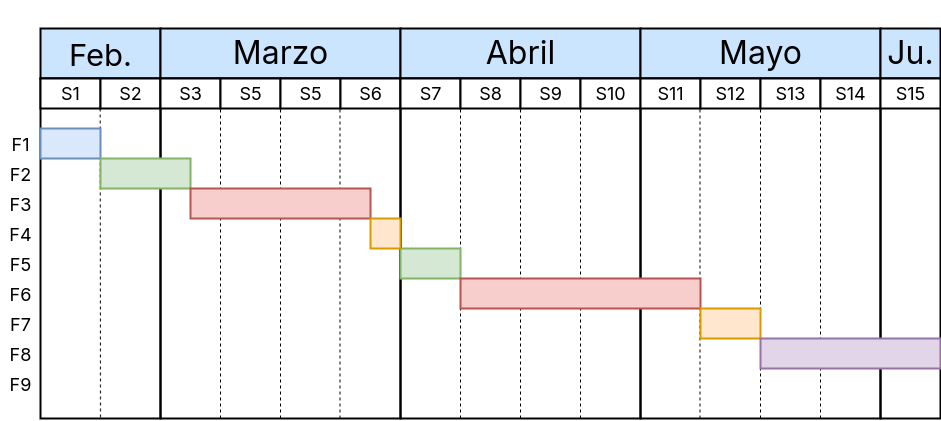
\includegraphics[width=\textwidth]{gantt.png}
	\caption{Diagrama de Gantt que muestra la organización de las distintas fases del proyecto a lo largo de las semanas.}
\end{figure}

\begin{itemize}
    \item La fase de color azul representa un breve análisis inicial de los requisitos, para resolver las dudas que puedan surgir acerca de los objetivos del trabajo.
    \item Las verdes corresponden al tiempo de diseño. En el caso del firmware conviene ser algo más generoso, teniendo en cuenta el tiempo de adaptación inicial al proyecto.
    \item Las secciones rojas son las de desarrollo.
    \item Las fases de pruebas vienen señaladas en color naranja, siendo la segunda un poco más extensa para poder hacer un repaso final.
    \item En morado está marcada la fase de documentación, que incluye tanto la del código como la generación de esta memoria.
\end{itemize}

Las tareas a realizar en cada fase serán detelladas más a fondo en sus capítulos correspondientes.

    
    \chapter{Firmware}
\label{ch:firmware}

\section{Análisis}
\label{sec:fw_analisis}

El primer paso para comenzar a trabajar en el firmware del dispositivo es realizar un análisis en el que se concreten los requisitos de las funcionalidade a incorporar al sistema.

Como se comentó en la sección \ref{sec:motivacion}, este proyecto es producto de las necesidades de Valeo, una empresa distribuidora de partes de vehículos. Junto a estas, pretenden también proporcionar a sus fabricantes herramientas para probar su correcto funcionamiento. Una de estas herramientas es el PWM Box.

En base a esto, se puede determinar que nuestro producto será usado principalmente en un entorno similar a una fábrica de coches o un taller mecánico. El perfil de su usuario principal será, por lo tanto, el de alguien que no necesariamente tenga conocimientos tecnológicos. Si se espera cierta familiaridad con dispositivos del entorno industrial, con controles similares al nuestro y una interfaz del mismo estilo.

Teniendo en cuenta las necesidades de la empresa y el perfil de este usuario, podemos definir los siguientes requisitos adicionales:

\clearpage

\subsubsection{Gestión de perfiles}

\begin{table}[h!]
    \centering
    \begin{tabular}{|m{2.5cm}|m{9.27cm}|}
        \hline
        \textbf{ID} & RF-1 \\
        \hline
        \textbf{Nombre} & Guardar perfiles \\
        \hline
        \textbf{Descripción} & El sistema debe permitir al usuario guardar la configuración activa en forma de perfil, que debe mantenerse en la memoria tras reiniciar el dispositivo. Esta operación debe estar protegida con contraseña, de forma que solo los usuarios autorizados puedan realizarla. \\
        \hline
        \textbf{Prioridad} & Alta \\
        \hline
    \end{tabular}
    \caption{RF-1. Guardar perfiles.}
\end{table}

\begin{table}[h!]
    \centering
    \begin{tabular}{|m{2.5cm}|m{9.27cm}|}
        \hline
        \textbf{ID} & RF-2 \\
        \hline
        \textbf{Nombre} & Cargar perfiles \\
        \hline
        \textbf{Descripción} & El sistema debe permitir al usuario cargar los perfiles almacenados en la memoria, estableciéndolos como activos. Esta operación debe estar protegida con contraseña, de forma que solo los usuarios autorizados puedan realizarla. \\
        \hline
        \textbf{Prioridad} & Alta \\
        \hline
    \end{tabular}
    \caption{RF-2. Cargar perfiles.}
\end{table}

\begin{table}[h!]
    \centering
    \begin{tabular}{|m{2.5cm}|m{9.27cm}|}
        \hline
        \textbf{ID} & RF-3 \\
        \hline
        \textbf{Nombre} & Eliminar perfiles \\
        \hline
        \textbf{Descripción} & El sistema debe permitir al usuario eliminar perfiles que estén actualmente almacenados en la memoria. Esta operación debe estar protegida con contraseña, de forma que solo los usuarios autorizados puedan realizarla. \\
        \hline
        \textbf{Prioridad} & Alta \\
        \hline
    \end{tabular}
    \caption{RF-3. Eliminar perfiles.}
\end{table}

\clearpage

\subsubsection{Gestión de la configuración del dispositivo}

\begin{table}[h!]
    \centering
    \begin{tabular}{|m{2.5cm}|m{9.27cm}|}
        \hline
        \textbf{ID} & RF-4 \\
        \hline
        \textbf{Nombre} & Guardar la contraseña \\
        \hline
        \textbf{Descripción} & El sistema debe almacenar la contraseña establecida en la memoria, de forma que esta se mantenga entre reinicios. \\
        \hline
        \textbf{Prioridad} & Alta \\
        \hline
    \end{tabular}
    \caption{RF-4. Guardar la contraseña.}
\end{table}

\begin{table}[h!]
    \centering
    \begin{tabular}{|m{2.5cm}|m{9.27cm}|}
        \hline
        \textbf{ID} & RF-5 \\
        \hline
        \textbf{Nombre} & Guardar el brillo de la pantalla \\
        \hline
        \textbf{Descripción} & Para la comodidad del usuario, el sistema debe almacenar la configuración de brillo del LCD en la memoria, de forma que esta se mantenga entre reinicios. \\
        \hline
        \textbf{Prioridad} & Media \\
        \hline
    \end{tabular}
    \caption{RF-5. Guardar el brillo de la pantalla.}
\end{table}

\subsubsection{Funcionalidad de señales lentas}

\begin{table}[h!]
    \centering
    \begin{tabular}{|m{2.5cm}|m{9.27cm}|}
        \hline
        \textbf{ID} & RF-6 \\
        \hline
        \textbf{Nombre} & Mostrar secuencias disponibles \\
        \hline
        \textbf{Descripción} & El sistema debe permitir al usuario consultar las secuencias lentas disponibles para ejecutar. Este menú debe ser independiente al resto del sistema. \\
        \hline
        \textbf{Prioridad} & Alta \\
        \hline
    \end{tabular}
    \caption{RF-6. Mostrar secuencias disponibles.}
\end{table}

\begin{table}[h!]
    \centering
    \begin{tabular}{|m{2.5cm}|m{9.27cm}|}
        \hline
        \textbf{ID} & RF-7 \\
        \hline
        \textbf{Nombre} & Ejecutar secuencias lentas \\
        \hline
        \textbf{Descripción} & El sistema debe permitir al usuario ejecutar las distintas secuencias lentas proporcionadas. \\
        \hline
        \textbf{Prioridad} & Alta \\
        \hline
    \end{tabular}
    \caption{RF-7. Ejecutar secuencias lentas.}
\end{table}

\begin{table}[h!]
    \centering
    \begin{tabular}{|m{2.5cm}|m{9.27cm}|}
        \hline
        \textbf{ID} & RF-8 \\
        \hline
        \textbf{Nombre} & Parar la ejecución de secuencias lentas \\
        \hline
        \textbf{Descripción} & El sistema debe permitir al usuario parar la ejecución de la secuencia activa en cualquier momento. \\
        \hline
        \textbf{Prioridad} & Alta \\
        \hline
    \end{tabular}
    \caption{RF-8. Parar la ejecución de secuencias lentas.}
\end{table}

\section{Diseño}
\label{sec:fw_diseño}

Al tratarse de un desarrollo en proceso, el diseño de la arquitectura general del sistema ya estaba realizado. En este aspecto, los cambios a realizar son los derivados de la redistribución del código de algunas partes, que como se determinó en la sección \ref{sec:inginv}, dificultaba la incorporación de nuevas características.

\subsection{Menús}

El principal aspecto a rediseñar está en la parte del sistema que muestra los distintos menús al usuario. La idea es separar la actual implementación de los distintos menús en archivos independientes.

Por un lado, se creará un archivo de control, que será al que se haga referencia desde el resto del programa para hacer operaciones como cambiar de menú, actualizar la pantalla, cambiar el brillo del LCD, etc. Cuando se llamen a funciones que dependan de la pantalla que esté activa en ese momento, él será el que se encargue de delegar la tarea al menú que corresponda.

Por otro lado, cada menú disponible tendrá un archivo separado en el que se implementarán como mínimo las versiones correspondientes de las 3 operaciones básicas (actualizar pantalla, girar \textit{rotary encoder} y pulsar \textit{rotary encoder}). Esto permite que, en menús que requieran funciones específicas (como será el caso del menú de señales lentas que se pretende añadir), estas funciones sólo sean accesibles desde el menú que coresponda.

En la figura \ref{fig:fw_modules} incluída más adelante podemos ver el resultado de esta división. Se destaca también la inclusión de un nuevo tipo de menú, el menú del sistema. Este se encargará de mostrar la secuencia de inicio y el salvapantallas, tareas que estaban antes también unificadas con el resto. También será útil una vez se incluya el almacenamiento de perfiles en la memoria, pues permitirá mostrar un aviso cuando se llene la memoria.

\subsection{Entrada/Salida}

Para la parte de entrada/salida, también se entontraban agrupadas algunas funciones que no estaban del todo relacionadas entre sí. A la vez, se prevee necesario añadir nuevas funcionalidades relacionadas con la comunicación por el puerto serie para integrar el dispositivo con la interfaz gráfica, así como para solucionar los problemas detectados en el \textit{rotary encoder}.

Es por ello que se ha decidido dividir también el código de esta parte en 3 archivos: uno para el puerto serie, otro para el codificador rotarorio, y un tercero para el manejo de eventos.

\subsubsection{Especificaciones acerca de la comunicación por el puerto serie}

Para realizar la comunicación con la interfaz gráfica, se necesitará definir un formato para los mensajes que intercambie esta con el dispositivo.

En primer lugar, conviene determinar de alguna forma el comienzo y el final de un mensaje, lo que nos permitirá evitar errores procesando datos indebidos. Para el comienzo común servirá cualquier carácter que no se vaya a usar en ningún otro punto del mensaje. En este caso, se ha elegido el acento circunflejo (\verb|^|). Para el final, bastará con enviar un retorno de línea (\verb|\n|).

A continuación, se definirá un formato general para los mensajes. Como en este caso se va a realizar la comunicación por el puerto serie, que no es especialmente rápido, se priorizará que los mensajes sean lo más cortos posibles. De esta forma, llegamos a la siguiente especificación:

\begin{center}
    {\fontfamily{cmtt}\selectfont\verb|^T,C(,P1,P2 ... ,Pn)\n|}
\end{center}

Donde:

\begin{itemize}
    \item\textit{T} representa el tipo de mensaje, indicando \textit{?} una petición y \textit{!} un envío de datos.
    \item\textit{C} será una de las siguientes opciones, dependiendo del contenido que se esté transmitiendo:
        \begin{itemize}
            \item\textit{@} servirá como saludo inicial para establecer la conexión entre ambas partes.
            \item\textit{i} para información general del dispositivo.
            \item\textit{c} para la contraseña.
            \item\textit{n} se usará antes de enviar ranuras de memoria, para indicar cuántas.
            \item\textit{s} para ranuras (Slots) de memoria.
            \item\textit{p} para señales PWM.
        \end{itemize}
    \item\textit{Px} serán los distintos parámetros, que dependerán del comando enviado y se encuentran documentados en el código.
% TODO: ¿Añadirlos aquí?
\end{itemize}

Por último, cabría plantear el uso de algún mecanismo de detección de errores. En este caso, dada la baja complejidad y urgencia de la transmisión, se ha optado por posponer este aspecto del diseño, a la espera de probar la comunicación y determinar de forma experimental la frecuencia de errores.

\subsection{Memoria EEPROM}

Para el manejo de la memoria EEPROM, cabe especificar qué datos será necesarios guardar, así como la la forma en la que se van a almacenar los mismos.

En primer lugar se definirán las siguientes unidades:

\begin{itemize}
    \item\textbf{PWM:} Representación de una señal PWM en la memoria. Consistirá de sus 4 parámetros principales (modo, frecuencia, ciclo y fase), así como un nombre identificativo (por ejemplo, "Intermitentes").
    \item\textbf{Slot:} Llamado así por ser la unidad en la que se compartimentalizará la memoria (ranuras), representa una forma de agrupar señales PWM. Permitirá al usuario definir distintos modelos de coches de forma que cada PWM esté destinado a probar un grupo distinto de luces de faros. Consistirá de 8 señales PWM y de un nombre identificativo. Se añadirá, además, una variable que indicará si la ranura está ocupada o no. Esto permitirá evitar borrados reales de memoria, prolongando su vida útil y disminuyendo el coste en cuanto a rendimiento de la escritura.
\end{itemize}

Otros parámetros que se necesitarán guardar, teniendo en cuenta los requisitos establecidos son:

\begin{itemize}
    \item\textbf{Valor de inicialización:} Servirá para determinar si la memoria contiene o no datos, ya que en caso de que no los contenga, necesitará ser inicializada con algunos valores por defecto.
    \item\textbf{Número de serie:} Número identificador del dispositivo.
    \item\textbf{Versión del hardware}.
    \item\textbf{Versión del software}.
    \item\textbf{Brillo de la pantalla:} Permitirá mantener el brillo establecido entre ejecuciones.
    \item\textbf{Ranura por defecto:} Indica la ranura de memoria que se cargará automáticamente al iniciar el PWM Box.
    \item\textbf{Contraseña:} Debido al entorno en el que se plantea usar el dispositivo, descrito en la sección \ref{sec:fw_analisis}, no se estima necesario encriptar la contraseña de ninguna forma.
\end{itemize}

Dada la capacidad del usuario de añadir, borrar y reemplazar ranuras de memoria según desee, se prevee la necesidad de algún mecanismo adicional para determinar qué ranuras mostrar en el menú principal del dispositivo. Con este fin, se incluirá también un vector auxiliar, que contendrá el índice de las ranuras de la memoria en el orden en el que se les muestra al usuario. Actúa, por así decirlo, como un traductor entre el índice de las ranuras visibles al usuario y el índice de las mismas internamente. Esto puede entenderse más fácilmente con una representación, que se incluye en la \autoref{fig:eeprom_operations}

\begin{figure}[h!]
    \centering
    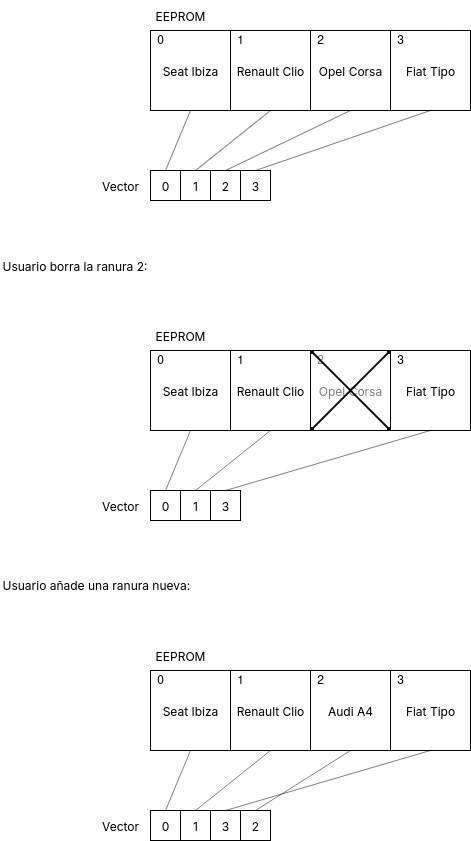
\includegraphics[width=0.8\textwidth]{eeprom_operations.png}
    \caption{Representación del funcionamiento del vector auxiliar al realizar distintas operaciones sobre la EEPROM.}
    \label{fig:eeprom_operations}
\end{figure}

\subsection{General}

La organización general de los archivos dentro del proyecto también se considera un aspecto importante a tener en cuenta para facilitar su manejo. Tras los cambios plantedos, algunos de los cuales incluyen la creación de aún más ficheros, esta necesidad se hace aún más aparente.

Para tratarlo, se plantea agruparlos en distintos directorios, a los que llamaremos módulos, de forma que queden distribuidos como se muestra en la figura \ref{fig:fw_modules}.

\begin{figure}[h!]
    \centering
	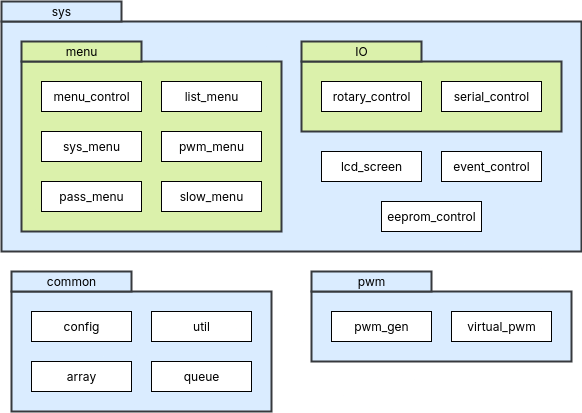
\includegraphics[width=\textwidth]{fw_modules.png}
	\caption{Distribución del código en distintos archivos y módulos.}
    \label{fig:fw_modules}
\end{figure}

\begin{itemize}
    \item\textbf{Módulo del sistema:} Contiene la implementación de características claves para el funcionamiento del sistema.
        \begin{itemize}
            \item\textbf{Módulo de E/S:} En él entontramos los archivos que definen el funcionamiento del \textit{rotary encoder} y de la UART, responsables de la comunicación con el usuario y la aplicación respectivamente.
            \item\textbf{Módulo de menús:} Agrupa la implementación de los distintos menús que usa el sistema.
        \end{itemize}
    \item\textbf{Módulo de PWM:} Se encarga de la generación y configuración de las señales de salida.
    \item\textbf{Módulo de archivos comunes:} Se tratan de utilidades genéricas, pensadas para ser usadas en común por las distintas partes del programa.
\end{itemize}

De esta forma, los distintos archivos quedan más agrupados según su funcionalidad, haciendo más viable establecer cierta encapsulación del código. Esto es especialmente importante teniendo en cuenta que el lenguaje con el que se trata no se especializa en la programación orientada a objetos, por lo que no permite definir clases al contrario que su sucesor. Podemos ver cómo quedaría la ejecución del bucle principal en la representación de la figura \ref{fig:fw_loop}. Adicionalmente, la figura \ref{fig:fw_interrupts} muestra el manejo de las interrupciones.

\begin{figure}[h!]
    \centering
    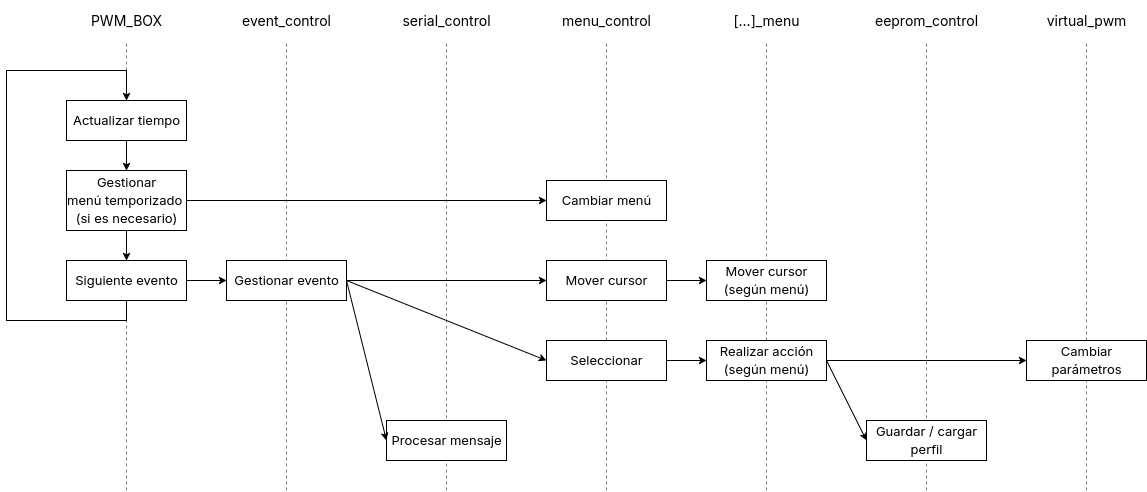
\includegraphics[width=\paperwidth,angle=-90,origin=c]{fw_loop.png}
    \caption{Ejecución del bucle principal.}
    \label{fig:fw_loop}
\end{figure}

\begin{figure}[h!]
    \centering
    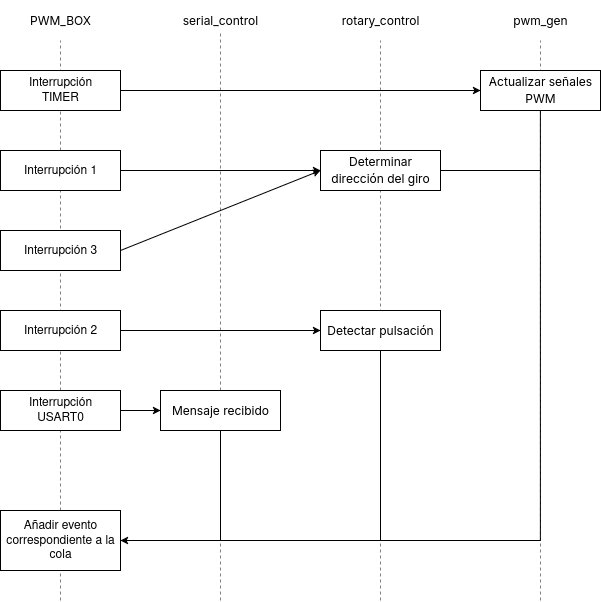
\includegraphics[width=\textwidth]{fw_interrupts.png}
    \caption{Ejecución de las distintas interrupciones.}
    \label{fig:fw_interrupts}
\end{figure}

\section{Desarrollo}

En esta sección se detallarán las decisiones enfrentadas durante la implementación del firmware, centrando la atención en los requerimientos definidos.

% Cabe destacar que también se ha realizado una extensa labor de limpieza del código, debido a una gran cantidad de declaraciones sin usar, definiciones redundantes y algunas prácticas que no se consideraban óptimas. En muchos casos, el código ha sido prácticamente reimplementando. Esto es, por supuesto, un aspecto subjetivo, por lo que no se hará referencia a ello nuevamente. Sin embargo, no mencionarlo sería subestimar el trabajo realizado en esta parte del proyecto.

Cabe mencionar, como regla general, que la mayoría sino todos los apartados incluidos en esta sección hacen uso de una forma u otra del \textit{datasheet} del ATmega 2560\cite{atmega2560}, microcontrolador incluido en el Arduino Mega 2560 del que se hace uso en este proyecto.

\subsection{Menú de señales lentas}

La funcionalidad de este menú se basa en un contador ejecutado en el bucle principal, que se incrementa cada medio segundo. Este es el máximo común divisor de la frecuencia con la que se actualizan estas señales. Cuando el usuario escoge una secuencia, este contador comienza a incrementarse, y a compararse en cada unidad con los instantes en los que la señal debe cambiar, los cuales se encuentran definidos en un \textit{switch}. Esto permite cambiar la señal a una frecuencia menor de la que el dispositivo soporta de base, pudiendo realizar pruebas en faros que así lo requieran.

Para que este menú sea independiente del resto del sistema, se ha implementado en el \textit{rotary encoder} la capacidad de detectar cuándo el botón ha sido mantenido (más detalles en la siguiente subsección). Cuando esto ocurra, el sistema mostrará esta pantalla.

\subsection{\textit{Rotary encoder}}

En este ámbito, el objetivo principal era el de corregir el funcionamiento algo errático del \textit{rotary encoder}. Sin embargo, la lógica del código presente no estaba del todo clara, por lo que se acabó reimplementando desde cero. Esto también ha permitido incluir la posibilidad de detectar pulsaciones largas del botón, como se ha mencionado en el apartado anterior.

\subsubsection{Pulsaciones}

El pin correspondiente del microcontrolador está programado para generar una interrupción en cada cambio de flanco. Esto, en el caso del botón, quiere decir que se generará una interrupción al pulsarse el mismo y otra al soltarse. En cada una, habrá por lo tanto que comprobar el estado del botón en ese instante. En caso de que se encuentre pulsado, se guardará en una variable ese instante de tiempo. Si por el contrario no está pulsado, se comparará la variable anterior con el instante actual (momento en el que termina la pulsación). De esta forma, se determina si el botón se ha pulsado o si se ha mantenido. Este será el resultado de la operación, cuyo evento correspondiente se añadirá al buffer en la rutina de la interrupción.

A esto se le añade una pequeña lógica de \textit{debouncing}, que sólo tendrá en cuenta cada pulsación si la anterior se ha realizado fuera de una breve ventana de tiempo. Esto evita la detección de pulsaciones duplicadas debido a inexactitudes en el circuito del codificador.

\subsubsection{Giros}

La lógica para el giro del \textit{rotary encoder} es más compleja. Debido al funcionamiento del mismo, la dirección de giro se puede determinar según \textbf{el orden} en el que dos pines emitan voltaje. De esta forma, determinando la secuencia de estados por los que pasan los pines al realizar giros para las dos direcciones, se puede crear una máquina de estados. Esta, comprobando el estado actual de los pines al manejarse la interrupción, determinará cuándo se ha completado una rotación. Al igual que en el caso anterior, cuando esto ocurra, se incluirá el evento correspondiente en la cola de eventos, que será procesado por el sistema.

Para seguir este método, también se programa el microcontrolador para que emita una interrupción en ambos flancos de ambos pines, y se va comparando su estado con el de la máquina de estados mencionada. Este funcionamiento se ha encontrado en la librería \url{https://github.com/buxtronix/arduino/tree/master/libraries/Rotary}, cuyo código fuente ha sido adaptado para funcionar en este proyecto.

% Un rotary encoder consiste de un disco giratorio sobre el que se distribuyen unas zonas de contacto. El disco suele conectarse a tierra, mientras que las zonas de contacto servirán para transmitir voltaje. Al girar el rotary encoder, ambos pines A y B harán contacto con una de las zonas brevemente, generándose un pulso representable como una señal cuadrada.

\subsection{Serial control}

Una de los factores más importantes para la comunicación del puerto serie es configurar correctamente los puertos del microcontrolador. En este caso, se han habilitado las interrupciones RX (para la recepción) y TX (para el envío) y se ha configurado la comunicación para usar 8-bits por segmento.

Una de las desventajas de usar el puerto seria para la comunicación, es que sus velocidades de transmisión no son especialmente altas. Por ello, se plantea activar el modo \textit{Double Speed Operation} del ATmega 2560 para llegar a 115200 baudios. Con este, el valor a establecer en el puerto UBBR vendrá dado por la siguiente ecuación: \cite{atmega2560}

\begin{center}
    \[UBBR = \frac{f_{OSC}}{8 \cdot BAUD} - 1\]
\end{center}

Habiendo configurado el microcontrolador, el resto de la implementación se basa en definir funciones básicas que accedan al registro UDR0. Posteriormente, se usan estan funciones para implementar el sistema de envío y recepcion de datos, ya cubiertos en la \ref{sec:fw_diseño}.

\subsection{Memoria EEPROM}

Esta parte se ha implementado utilizado el apoyo de la librería \verb|avr/eeprom.h|, que proporciona la directiva \verb|EEMEM|, la cual permite declarar variables en la memoria EEPROM. Estas, sin embargo, solo sirven para poder hacer referencia a la dirección de memoria en la que se encuentran los datos desde el programa. Para leer su valor o escribir en ellas, es necesario usar las funciones proporcionadas por la misma librería. Por ello, la mayoría de funciones incluídas en esta parte no son más que distintos \textit{getters} y \textit{setters} para las distintas variables determinadas en la sección \ref{sec:fw_diseño}.

A estas se une el vector auxiliar tambien mencionado en la sección \ref{sec:fw_diseño}. Para facilitar su manejo y hacer el código más reutilizable, se ha implementado una pequeña librería que define las funciones básicas esperables de un vector.

Con todo esto, el contenido de la memoria EEPROM puede verse en la \autoref{fig:eeprom_vars}.

\begin{figure}[h!]
    \centering
    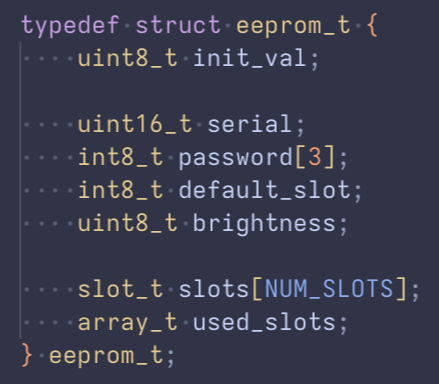
\includegraphics[width=0.5\textwidth]{eeprom_vars.png}
    \caption{Contenido de la memoria EEPROM.}
    \label{fig:eeprom_vars}
\end{figure}

\section{Pruebas}

Debido a la naturaleza del trabajo, la mayoría de pruebas se han realizado de manera experimental, observando los efectos de los cambios realizados sobre los distintos elementos.

Para comprobar que no se ha alterado la capacidad del dispositivo de emitir las señales de manera correcta, así como validar la implementación de las señales lentas, se ha usado un analizador lógico. En la figura \ref{fig:fw_pwm_signals} se muestran las señales PWM resultantes de distintas configuraciones. Adicionalmente, en las figuras \ref{fig:fw_slow_signal1} y \ref{fig:fw_slow_signal2}, se ven dos de las secuencias de señales lentas incluídas con el dispositivo.

\begin{figure}[h!]
    \centering
    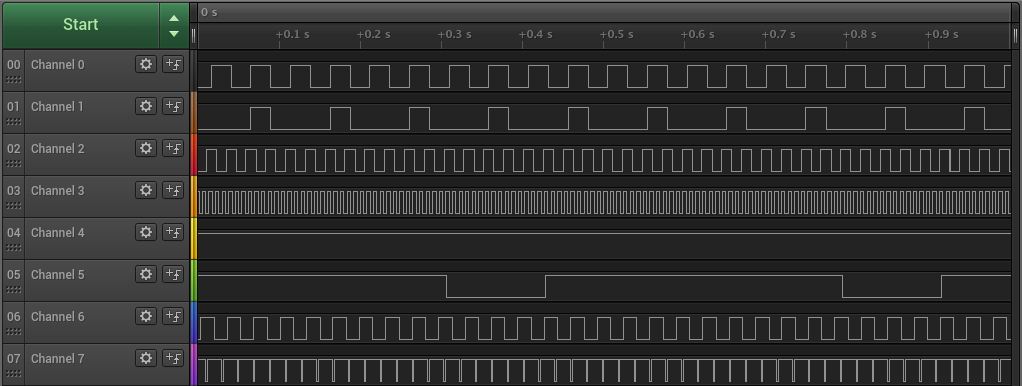
\includegraphics[width=\textwidth]{fw_pwm_signals.png}
    \caption{Señales PWM con distintas configuraciones.}
    \label{fig:fw_pwm_signals}
\end{figure}

\begin{figure}[h!]
    \centering
    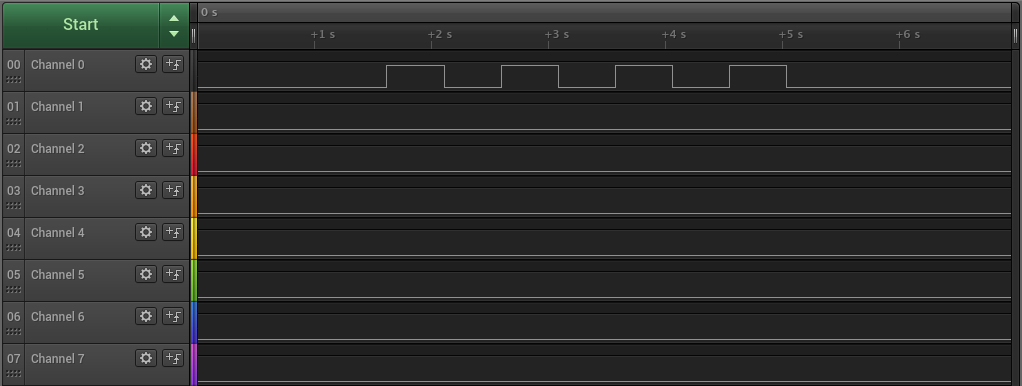
\includegraphics[width=\textwidth]{fw_slow_signal1.png}
    \caption{Una de las secuencias de señales lentas preconfiguradas.}
    \label{fig:fw_slow_signal1}
\end{figure}

\begin{figure}[h!]
    \centering
    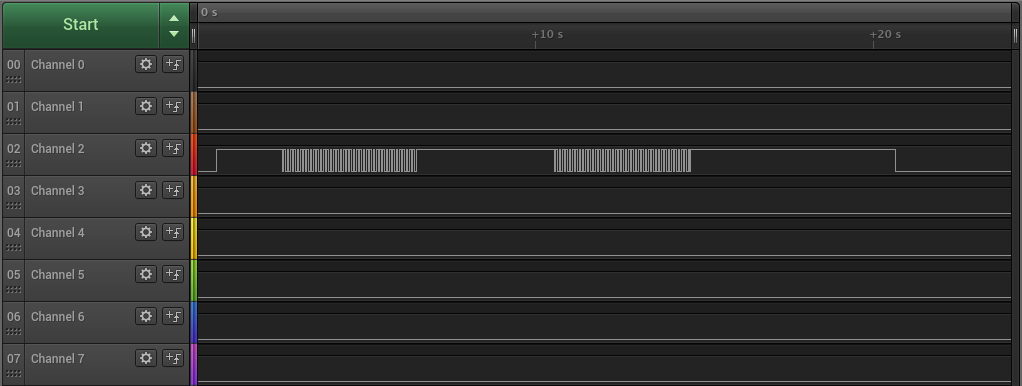
\includegraphics[width=\textwidth]{fw_slow_signal2.png}
    \caption{Otra de las secuencias de señales lentas preconfiguradas.}
    \label{fig:fw_slow_signal2}
\end{figure}

Estas pruebas han sido realizado con el Saleae Logic v1.2.40\footnote{https://support.saleae.com/logic-software/legacy-software/older-software-releases. Accedido el 28 de agosto de 2025.}, que es \textit{software} propietario. Sin embargo, también podría usarse una versión \textit{open-source} como puede ser Sigrok PulseView v0.4.2\footnote{https://sigrok.org/wiki/Downloads. Accedido el 28 de agosto de 2025.}.

% TODO: Medir con el PulseView


    \chapter{Interfaz gráfica}
\label{ch:ui}

\section{Análisis}

En esta sección se comenzará a trabajar en la aplicación, realizando en primer lugar un breve análisis para concretar sus requisitos.

En el caso de la interfaz gráfica, el ámbito de uso difiere un poco del concretado para el firmware en la \autoref{sec:fw_analisis}. Esta se pretende usar desde Valeo para incluir en el dispositivo las ranuras que cada fabricante necesite antes de proporcionarles el PWM Box. Por lo tanto, se deduce que su uso va a ser en un entorno algo más administrativo que en el caso anterior.

Si bien se anticipa, por lo tanto, que el usuario tenga un mayor nivel de entendimiento a la hora de manejar sistemas informáticos, sigue sin esperarse ningún tipo de conocimiento técnico. Solamente se asumirá algo de destreza en el uso de programas de ofimática y similares.

Teniendo esto en cuenta, se determinarán los requisitos de la aplicación.

\subsubsection{Comunicación con el dispositivo}

\begin{table}[h!]
    \centering
    \begin{tabular}{|m{2.5cm}|m{9.27cm}|}
        \hline
        \textbf{ID} & RF-1.1 \\
        \hline
        \textbf{Nombre} & Conectar con el dispositivo \\
        \hline
        \textbf{Descripción} & El sistema debe ser capaz de encontrar el puerto del dispositivo en el equipo y conectarse a él de forma automática, tanto desde Windows como desde Linux. \\
        \hline
        \textbf{Prioridad} & Alta \\
        \hline
    \end{tabular}
    \caption{RF-1.1. Conectar con el dispositivo.}
\end{table}

\begin{table}[h!]
    \centering
    \begin{tabular}{|m{2.5cm}|m{9.27cm}|}
        \hline
        \textbf{ID} & RF-1.2 \\
        \hline
        \textbf{Nombre} & Obtener la información básica del dispositivo \\
        \hline
        \textbf{Descripción} & El sistema debe poder obtener la información básica del dispositivo. Esto incluye su número de serie, su versión de \textit{hardware} y su versión de \textit{software}. \\
        \hline
        \textbf{Prioridad} & Alta \\
        \hline
    \end{tabular}
    \caption{RF-1.2. Obtener la información básica del dispositivo.}
\end{table}

\begin{table}[h!]
    \centering
    \begin{tabular}{|m{2.5cm}|m{9.27cm}|}
        \hline
        \textbf{ID} & RF-1.3 \\
        \hline
        \textbf{Nombre} & Obtener la configuración general del dispositivo \\
        \hline
        \textbf{Descripción} & El sistema debe tener la capacidad de obtener la configuración general del dispositivo, que consiste de su contraseña y la ranura por defecto establecida. \\
        \hline
        \textbf{Prioridad} & Alta \\
        \hline
    \end{tabular}
    \caption{RF-1.3. Obtener la configuración general del dispositivo.}
\end{table}

\begin{table}[h!]
    \centering
    \begin{tabular}{|m{2.5cm}|m{9.27cm}|}
        \hline
        \textbf{ID} & RF-1.4 \\
        \hline
        \textbf{Nombre} & Obtener las ranuras guardadas en el dispositivo \\
        \hline
        \textbf{Descripción} & El sistema debe comunicarse con el dispositivo para obtener las ranuras que estén guardadas en la memoria del mismo, incluyendo la información relativa a las señales PWM que las componen. \\
        \hline
        \textbf{Prioridad} & Alta \\
        \hline
    \end{tabular}
    \caption{RF-1.4. Obtener las ranuras guardadas en el dispositivo.}
\end{table}

\begin{table}[h!]
    \centering
    \begin{tabular}{|m{2.5cm}|m{9.27cm}|}
        \hline
        \textbf{ID} & RF-1.5 \\
        \hline
        \textbf{Nombre} & Enviar configuración general al dispositivo \\
        \hline
        \textbf{Descripción} & El sistema debe ser capaz de enviar de vuelta al dispositivo su configuración básica. \\
        \hline
        \textbf{Prioridad} & Alta \\
        \hline
    \end{tabular}
    \caption{RF-1.5. Enviar configuración general al dispositivo.}
\end{table}

\begin{table}[h!]
    \centering
    \begin{tabular}{|m{2.5cm}|m{9.27cm}|}
        \hline
        \textbf{ID} & RF-1.6 \\
        \hline
        \textbf{Nombre} & Enviar ranuras al dispositivo \\
        \hline
        \textbf{Descripción} & El sistema debe poder enviar ranuras configuradas al dispositivo. \\
        \hline
        \textbf{Prioridad} & Alta \\
        \hline
    \end{tabular}
    \caption{RF-1.6. Enviar ranuras al dispositivo.}
\end{table}

\subsubsection{Gestión del dispositivo}

\begin{table}[h!]
    \centering
    \begin{tabular}{|m{2.5cm}|m{9.27cm}|}
        \hline
        \textbf{ID} & RF-2.1 \\
        \hline
        \textbf{Nombre} & Mostrar la información básica del dispositivo \\
        \hline
        \textbf{Descripción} & El sistema debe permitir al usuario consultar la información básica del dispositivo. \\
        \hline
        \textbf{Prioridad} & Alta \\
        \hline
    \end{tabular}
    \caption{RF-2.1. Mostrar la información básica del dispositivo.}
\end{table}

\begin{table}[h!]
    \centering
    \begin{tabular}{|m{2.5cm}|m{9.27cm}|}
        \hline
        \textbf{ID} & RF-2.2 \\
        \hline
        \textbf{Nombre} & Mostrar la configuración general del dispositivo \\
        \hline
        \textbf{Descripción} & El sistema debe al usuario visualizar la configuración general del dispositivo. \\
        \hline
        \textbf{Prioridad} & Alta \\
        \hline
    \end{tabular}
    \caption{RF-2.2. Mostrar la configuración general del dispositivo.}
\end{table}

\begin{table}[h!]
    \centering
    \begin{tabular}{|m{2.5cm}|m{9.27cm}|}
        \hline
        \textbf{ID} & RF-2.3 \\
        \hline
        \textbf{Nombre} & Modificar la configuración general del dispositivo \\
        \hline
        \textbf{Descripción} & El sistema debe permitir al usuario establecer una nueva contraseña y definir cuál será la ranura cargada por defecto. \\
        \hline
        \textbf{Prioridad} & Alta \\
        \hline
    \end{tabular}
    \caption{RF-2.3. Mostrar la configuración general del dispositivo.}
\end{table}

\subsubsection{Gestión de ranuras}

\begin{table}[h!]
    \centering
    \begin{tabular}{|m{2.5cm}|m{9.27cm}|}
        \hline
        \textbf{ID} & RF-3.1 \\
        \hline
        \textbf{Nombre} & Crear ranuras nuevas \\
        \hline
        \textbf{Descripción} & El sistema debe permitir al usuario crear ranuras nuevas. \\
        \hline
        \textbf{Prioridad} & Alta \\
        \hline
    \end{tabular}
    \caption{RF-3.1. Crear ranuras nuevas.}
\end{table}

\begin{table}[h!]
    \centering
    \begin{tabular}{|m{2.5cm}|m{9.27cm}|}
        \hline
        \textbf{ID} & RF-3.2 \\
        \hline
        \textbf{Nombre} & Exportar ranuras al equipo \\
        \hline
        \textbf{Descripción} & El sistema debe permitir exportar las ranuras cargadas a la memoria del equipo en un formato adecuado. \\
        \hline
        \textbf{Prioridad} & Alta \\
        \hline
    \end{tabular}
    \caption{RF-3.2. Exportar ranuras al equipo.}
\end{table}

\begin{table}[h!]
    \centering
    \begin{tabular}{|m{2.5cm}|m{9.27cm}|}
        \hline
        \textbf{ID} & RF-3.3 \\
        \hline
        \textbf{Nombre} & Importar ranuras del equipo \\
        \hline
        \textbf{Descripción} & El sistema debe permitir al usuario importar las ranuras almacenadas con un determinado formato en la memoria del equipo. \\
        \hline
        \textbf{Prioridad} & Alta \\
        \hline
    \end{tabular}
    \caption{RF-3.3. Importar ranuras del equipo.}
\end{table}

\begin{table}[h!]
    \centering
    \begin{tabular}{|m{2.5cm}|m{9.27cm}|}
        \hline
        \textbf{ID} & RF-3.4 \\
        \hline
        \textbf{Nombre} & Visualizar la configuración de las ranuras \\
        \hline
        \textbf{Descripción} & El sistema permitir al usuario consultar los parámetros de las señales PWM que componen las ranuras cargadas. \\
        \hline
        \textbf{Prioridad} & Alta \\
        \hline
    \end{tabular}
    \caption{RF-3.4. Visualizar la configuración de las ranuras.}
\end{table}

\begin{table}[h!]
    \centering
    \begin{tabular}{|m{2.5cm}|m{9.27cm}|}
        \hline
        \textbf{ID} & RF-3.5 \\
        \hline
        \textbf{Nombre} & Modificar los parámetros de las ranuras cargadas \\
        \hline
        \textbf{Descripción} & El sistema debe permitir la creación de ranuras nuevas desde la propia aplicación. \\
        \hline
        \textbf{Prioridad} & Alta \\
        \hline
    \end{tabular}
    \caption{RF-3.5. Obtener las ranuras guardadas en el dispositivo.}
\end{table}

\section{Diseño}

La fase de diseño de la interfaz se comienza con un repaso de los requisitos. Teniendo en cuenta que su objetivo principal es ser usada en la industria automobilística, desde el comienzo del diseño se planteó un producto simple, con la mayor cantidad de información posible a simple vista.



Esta idea inicial fue variando ligeramente conforme fuimos concretando algunas de las características a implementar, pero siempre se mantuvo fiel a su diseño original.

El resultado final


\subsection{JSON Manager}



\subsection{PWM Types}



\subsection{PWM Box}



\subsection{Main Window}




\section{Desarrollo}



\section{Pruebas}




    \bibliographystyle{bababbrv-fl}
    \bibliography{bibliografia}

    % \nocite{*}
    % \bibliography{bibliografia/bibliografia}\addcontentsline{toc}{chapter}{Bibliografía}

    \appendix

    \chapter*{}
    \thispagestyle{empty}

\end{document}
